%%%%%%%%%%%%%%%%%%%%%%%%%%%%%%%%%%%%%%%%%
% University/School Laboratory Report
% LaTeX Template
% Version 3.1 (25/3/14)
%
% This template has been downloaded from:
% http://www.LaTeXTemplates.com
%
% Original author:
% Linux and Unix Users Group at Virginia Tech Wiki 
% (https://vtluug.org/wiki/Example_LaTeX_chem_lab_report)
%
% License:
% CC BY-NC-SA 3.0 (http://creativecommons.org/licenses/by-nc-sa/3.0/)
%
%%%%%%%%%%%%%%%%%%%%%%%%%%%%%%%%%%%%%%%%%

%----------------------------------------------------------------------------------------
%	PACKAGES AND DOCUMENT CONFIGURATIONS
%----------------------------------------------------------------------------------------

\documentclass{article}

\usepackage{graphicx} % Required for the inclusion of images
\usepackage{natbib} % Required to change bibliography style to APA
%\usepackage{biblatex}

\setlength\parindent{0pt} % Removes all indentation from paragraphs

\renewcommand{\labelenumi}{\alph{enumi}.} % Make numbering in the enumerate environment by letter rather than number (e.g. section 6)
\usepackage{algorithm,amsmath,algpseudocode}
\usepackage{float}
%\usepackage{times} % Uncomment to use the Times New Roman font


%----------------------------------------------------------------------------------------
%	DOCUMENT INFORMATION
%----------------------------------------------------------------------------------------

\title{Active Learning for Image Classification \\ Automation of Biological Research \\ Final Report} % Title

\author{Ruijian \textsc{Wang}, Jianhe \textsc{Luo}} % Author name

\date{\today} % Date for the report

\begin{document}

\maketitle % Insert the title, author and date

% \begin{center}
% \begin{tabular}{l r}
% Date Performed: & December 13, 2015 \\ % Date the experiment was performed
% Partners: & Ruijian Wang \\ % Partner names
% & Jianhe Luo \\
% Instructor: & Professor Langmead % Instructor/supervisor
% \end{tabular}
% \end{center}

% If you wish to include an abstract, uncomment the lines below
% \begin{abstract}
% Abstract text
% \end{abstract}

%Introduction
%Background and Related Work
%Methods
%Experiments and Results
%Discussion
%Conclusions and Future Work
%References

%----------------------------------------------------------------------------------------
%	SECTION 1
%----------------------------------------------------------------------------------------

\section{Introduction}

Image classification is not a new research area, but it is still a major challenge because of the nature of image. One challenge is a lot of labeled training examples required. It is both time and cost consuming to label a good set of images, especially for medical image. Active learning has attracted a lot of attention since it can select the `useful' observation by some strategy. So that manual effort can focus on labeling the most helpful examples to build a machine learning model. In this paper, we tried to select the informational examples from different views and apply them in different situations.


%\begin{center}\ce{2 Mg + O2 -> 2 MgO}\end{center}

% If you have more than one objective, uncomment the below:
%\begin{description}
%\item[First Objective] \hfill \\
%Objective 1 text
%\item[Second Objective] \hfill \\
%Objective 2 text
%\end{description}

%\subsection{Definitions}
%\label{definitions}
%\begin{description}
%\item[Stoichiometry]
%The relationship between the relative quantities of substances taking part in a reaction or forming a compound, typically a ratio of whole integers.
%\item[Atomic mass]
%The mass of an atom of a chemical element expressed in atomic mass units. It is approximately equivalent to the number of protons and neutrons in the atom (the mass number) or to the average number allowing for the relative abundances of different isotopes. 
%\end{description} 
 
%----------------------------------------------------------------------------------------
%	SECTION 2
%----------------------------------------------------------------------------------------

\section{Background and Related Work}
Although many researches have been devoted to image classification, however, only a few of them are related to the medical domain. More and more attention have been paid to medical image classification\textbf{citation}. Many machine learning algorithms have been applied to medical image classification, including the large margin classifiers, decision trees and neural networks. Among all of the algorithms, the support vector machine(\textbf{SVM}) and kernel logistic regression(\textbf{KLR}) appeared to be the most effective methods\cite{hoi2006batch}.

\subsection{Data Source}
The data set is composed of 5120 unlabeled images. All the images are represented by a 26-dimension vector, which are already being processed. There are 8 classes for those images and are represented by 1,2,3,4,5,6,7,8.
\subsection{Pool-based learning setup}
Pool-based learning task is very common for active learning. Start with a small amount of training observations that are selected randomly, we get a seed set and a naive machine learning model, based on the naive machine learning model and candidate observation pool, we select new observation(s) along with the query result, adding to the training set to retrain the model. The selection process is iterative such that after each iteration of model's prediction and relevant parameters, we select new observation to improve the model. Every time we call the oracle(query the label from expert), we will calculate the loss value for the entire data set until all queries are consumed. Compare the selection strategy with random selector by plotting the loss value graph.
\subsection{Stream-based learning setup}
%\begin{tabular}{ll}
%Mass of empty crucible & \SI{7.28}{\gram}\\
%Mass of crucible and magnesium before heating & \SI{8.59}{\gram}\\
%Mass of crucible and magnesium oxide after heating & \SI{9.46}{\gram}\\
%Balance used & \#4\\
%Magnesium from sample bottle & \#1
%\end{tabular}

\subsection{Difference between pool-based and stream-based}
For the pool based learning process, we see all the unlabeled data referred as the active pool. The advantage by seeing all the data is we can rank the data or use the structure of the data \cite{dasgupta2008hierarchical}, and then select the useful observation(s). 
While for the stream based learning process, the restriction is we only know the current input data, and all the previous data if you cached them. That prevents us from using ranking techniques and we need to make decision based on the current model and the input observation.
%----------------------------------------------------------------------------------------
%	SECTION 3
%----------------------------------------------------------------------------------------

\section{Methods}

%\begin{tabular}{ll}
%Mass of magnesium metal & = \SI{8.59}{\gram} - \SI{7.28}{\gram}\\
%& = \SI{1.31}{\gram}\\
%Mass of magnesium oxide & = \SI{9.46}{\gram} - \SI{7.28}{\gram}\\
%& = \SI{2.18}{\gram}\\
%Mass of oxygen & = \SI{2.18}{\gram} - \SI{1.31}{\gram}\\
%& = \SI{0.87}{\gram}
%\end{tabular}
\subsection{Data distribution} \label{data_distribution}
We can get a overview of the distribution of all the labels. From the following graph we can see almost each label has equal amount of observations. Thus we can make a assumption that when we randomly select the seed set data, each label will be covered.
\begin{figure}
\centering
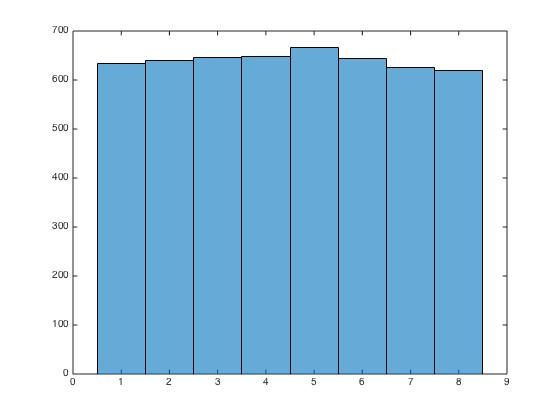
\includegraphics[scale=0.5]{label_distribution}  
\caption{All data's label distribution}
\end{figure}
\subsection{Pool-based learning}

\subsubsection{Random learner}
The random learner is designed to be compared with some selection strategy. The logic for random learner is quite simple.

\begin{algorithm}[H]
	\caption{Random selection for pool based learning}
	\begin{algorithmic}
		\State Randomly choose 50 observations as seed set
		\State Train the initial SVM models with seed set
		\While {$oracle_num \leq 462$} 
			Randomly select an observation.
			
			Add it to the training data and remove it from candidate pool. 
			
			Retrain the 8 binary classifiers.
		\EndWhile
	\State Plot the loss value
	\end{algorithmic}
\end{algorithm}

\subsubsection{Query from committee}
The Expected Loss Optimization \cite{long2010active} is a straight-forward strategy. Since we got 8 labels from all the data and we will use 8 binary classifiers to help us select the informative observation, each classifier is a binary \textbf{SVM} classification model. For the first binary classifier, we will set data with label 1 as positive observations and choose equal number of data with other labels as negative data. Similarly, for the second and following classifiers, we will set label 2,3...8 as positive observations accordingly, and set observations with other labels as negative observations. By selecting the seed set, we got the initial training data set and get 8 binary classifiers.
\\
\\
Based on the 8 binary classifiers, we can get a $1\times 8$ vector for each observation, after processed, the value in the vector with value 1 means the classifier of this index make a positive prediction. The sum of the vector is the total number of binary classifiers predict positively. Select the observation with most positive results. Since the sum result ranges from 0 to 9, and we have 5120 observations, it will be very likely to have more than one observation with same number of positive results. Among all the observations with most positive predictions, we can apply another selection strategy. For simplicity, we just randomly pick up one of them and add it to the training data.
\\
\\
After each iteration, calculate the loss value and plot the loss value after finishing all the iterations.

\begin{algorithm}[H]
	\caption{Query from committee pool based learning}
	\begin{algorithmic}
		\State Randomly choose 50 observations as seed set
		\State Train the initial SVM models with seed set
		\While {$oracle_num \leq 462$} 
		
			Predict all the observations and get a $N \times 8$ matrix.

			Sum each observation's positive prediction number.
			
			Rank based on the number of positive prediction number
			
			Choose the observation with most positive predictions
			
			Add it to the training data and remove it from candidate pool.
			
			Retrain the 8 binary classifiers.
		\EndWhile
	\State Plot the loss value
	\end{algorithmic}
\end{algorithm}
%Because of this reaction, the required ratio is the atomic weight of magnesium: \SI{16.00}{\gram} of oxygen as experimental mass of Mg: experimental mass of oxygen or $\frac{x}{1.31}=\frac{16}{0.87}$ from which, $M_{\ce{Mg}} = 16.00 \times \frac{1.31}{0.87} = 24.1 = \SI{24}{\gram\per\mole}$ (to two significant figures).



\subsubsection{Entropy Measure}
The entropy measure\cite{joshi2009multi} strategy is select the observation with largest entropy. Unlike the query from committee strategy, we use multi-class Naive Bayes model for this selection strategy since we need the posterior probability for each label.

After training the initial model by seed set, estimate the posterior probability of each label for every observation, we can get entropy for each observation, and rank by the entropy.

\begin{algorithm}[H]
	\caption{Entropy Measure for pool based learning}
	\begin{algorithmic}
		\State Randomly choose 50 observations as seed set
		\State Train the initial multi-calss Naive Bayes model with seed set
		\While {$oracle_num \leq 462$} 
		
			Predict all the observations and get a $N \times 8$ matrix.

			Estimate the posterior probability of each label for each observation.
	
			Calculate the entropy based on posterior probability.
			
			Sum each observation's entropy
			
			Rank based on the sum of entropy.
			
			Choose the observation with largest entropy.
			
			Add it to the training data and remove it from candidate pool.
			
			Retrain the multi-class Naive Bayes classifier.
		\EndWhile
	\State Plot the loss value
	\end{algorithmic}
\end{algorithm}

\subsection{Stream-based learning}

\subsubsection{Random learner}
There are two kinds of random learner, first random learner only contains a multi-class SVM model, and second random learner only contains 8 binary classifiers.
\begin{algorithm}[H]
	\caption{First random learner for stream-based learning}
	\begin{algorithmic}
		\State Randomly choose 10 observations as seed set
		\State Train the initial multi-calss SVM model with seed set
		\For {$i = 1:oracle_nums$}

			Get next image.
			
			Add the new image to training data set.
			
			Retrain the model.
			
			Test error.
		\EndFor
		
	\State Plot error values
	\end{algorithmic}
\end{algorithm}

\begin{algorithm}[H]
	\caption{Second random learner for stream-based learning}
	\begin{algorithmic}
		\State Randomly choose 10 observations as seed set
		\State Construct the training data and train 8 initial binary SVM models
		\For {$i = 1:oracle_nums$}

			Get next image.
			
			Add the new image to training data set.
			
			Retrain the model.
			
			Test error.
		\EndFor
		
	\State Plot error values
	\end{algorithmic}
\end{algorithm}
\subsubsection{Query from committee}
Based on our mid-term report, we make some improvement for our model. Previously, there are only 8 binary classifiers and all prediction came from the 8 binary classifiers predictions.
\\
\\
We add another multi-class classifier, use its predictions as the main result and assisted by the 8 binary classifiers' predictions.

\begin{algorithm}[H]
	\caption{Query from committee stream-based learning}
	\begin{algorithmic}
		\State Randomly choose 10 observations as seed set
		\State Construct the training data and train 8 initial binary SVM models and one multi-class model.
		\For $i = 1:5120$
			\State Get prediction vector from binary classifiers referred as binary predictions.
			\State Get prediction from the multi-class classifier referred as overall prediction.
			\If {there are more than one positive predictions in binary predictions}
				\State Choose the overall prediction as final result
			\ElsIf {there are no positive predictions in binary predictions}
				\State \textbf{Call oracle}, add this observation to training data.
				\State Get Testset Error
				\State Choose the overall prediction as final result
			\Else \Comment {only one positive}
				\State Choose the positive binary prediction as final result.
			\EndIf
		\EndFor\\
		\Return {number of oracle calls, testset error}
	\end{algorithmic}
\end{algorithm}


%----------------------------------------------------------------------------------------
%	SECTION 4
%----------------------------------------------------------------------------------------

\section{Experiments and Results}

\subsection{Pool-based learning}
For the pool based active learning task, we first randomly select 50 observations as seed set, and at each iteration, select the most useful observation and repeat 462 times since only 512 oracle calls are allowed.
\subsubsection{Query from committee selection strategy}
To test the assumption we made at \ref{data_distribution}, we plot the label distribution of seed set.
\begin{figure}[H]
\centering
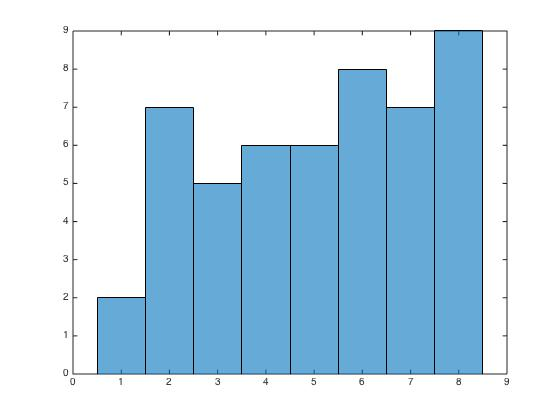
\includegraphics[scale=0.5]{posterior_train_distribution}
\caption{Seed set's label distribution}
\end{figure}

Run two different active learning process, query form committee and random selection, plot the result function.
\begin{figure}[H]
\centering
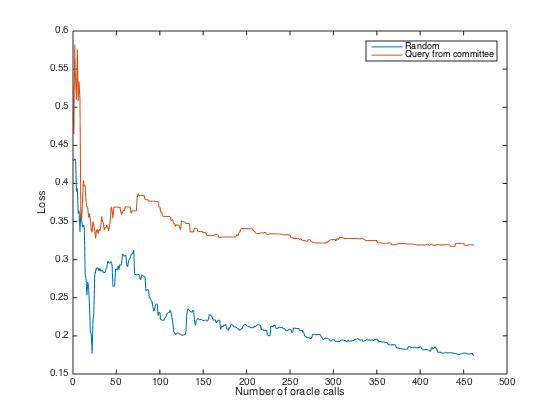
\includegraphics[scale=0.5]{loss_optimize_vs_random_pool_based}
\caption{Loss Optimize and Random Learner}
\end{figure}
From the graph we can see the loss optimize selection strategy does not perform well. Although it converges at last but the loss value is almost twice as random learner.

To test my guess, I even select the observation the other way around, always select the one with minimum positive predictions, it turns out it also converges at similar loss value.
\begin{figure}[H]
\centering
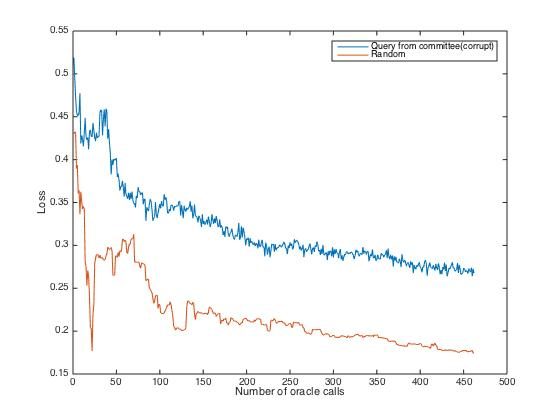
\includegraphics[scale=0.5]{pool_based_loss_rank_corrupt_random}
\caption{Corrupt Loss Optimize and Random Learner}
\end{figure}
From the graph we can see, the loss value still goes down but it will keep fluctuating.Those two graphs proves that this strategy is not a good active learning strategy.

\subsubsection{Entropy Measure selection strategy}
\begin{figure}[H]
\centering
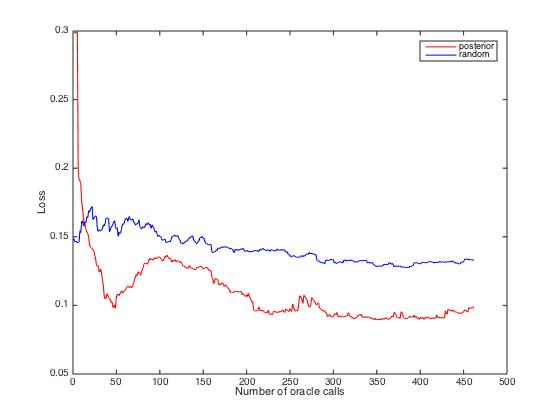
\includegraphics[scale=0.5]{posterior_vs_random_pool_based}
\caption{Loss value of entropy measure and random learner}
\end{figure}
From the graph we can see, the random learner has a lower loss value at the very beginning, however, the seed set is selected randomly, the beginning loss value means nothing. After around 10 iteration, the query from committee selection strategy has reached a lower loss value and keep reducing quickly. And finally reached around 0.1 loss value, lower than the random learner loss value, which is around 0.14.
%\begin{figure}[h]
%\begin{center}
%
\includegraphics[width=0.65\textwidth]{placeholder} % Include the image placeholder.png
%\caption{Figure caption.}
%\end{center}
%\end{figure}
\subsection{Stream-based learning}
For stream based learning, after finish the initial machine learning model, execute 5120 times for-loop, record the number of oracle calls and select the useful observation for each loop. Each time call the oracle, calculate the test set error. After execution, run random learners based on number of oracle calls, calculate the test set error, plot the test set error to compare performance.

\begin{figure}[H]
\centering
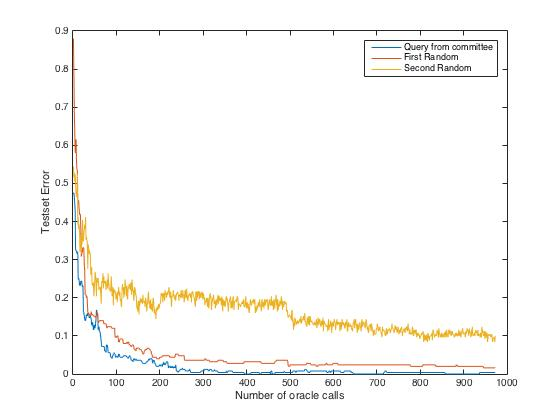
\includegraphics[scale=0.5]{stream-based-overall-result} \label{stream-based-result}
\caption{Stream based learner and two random learner}
\end{figure}

From the graph we can see our active learning strategy do achieve better performance than two random learner. The first random learner, which only contains 8 binary classifiers has higher error. It is consistent with the pool-based query from committee results.
%----------------------------------------------------------------------------------------
%	SECTION 5
%----------------------------------------------------------------------------------------

\section{Discussion}
The result of query from committee in pool based is not a good selection strategy,  \ref{stream-based-result} shows that the second random leaner has significantly lower error value, and the second one only contains one multi-class classifier, which proves that our one-versus-all ensemble classifiers are not a good selection strategy.
\\
\\
Also the steam based task converges faster than pool based task, it usually takes 100 iterations for the former one and 300 iterations for the latter one. It is also a interesting result. One possible reason might be pool based learning task selects the observation without replacement. And iteration of stream based might select duplicated observation. Some already selected observation might still be helpful to improve the model, while in pool based non-replacement selection strategy, it cannot select the same observation. So the model can only choose the second most helpful observation to improve the model, which causes the model converges slower.

%----------------------------------------------------------------------------------------
%	SECTION 6
%----------------------------------------------------------------------------------------

\section{Conclusions and Future Work}
In this paper, we proposed different active learning strategy for both pool-based learning and stream-based learning. Through the results of those active learning model, it proves that active learning can reduce notable number of required training examples and achieve better performance at the same time.
\\
\\
For the future, we may try more complex ensemble model since the pool-based query from committee strategy does not work well and one of the potential problems might be that we just use linear number of binary classifiers and also the way we construct training data after seed set are selected. Because the one-versus-one approach \cite{hsu2002comparison} shows good classification performance. In the future, we might change the one versus all to one versus one method to test the performance.
\\
\\
Also there are too many oracle calls in steam based task, we tried Linear and Quadratic Discriminant Analysis, this model will call almost twice times oracle as SVM. It forces us to change the strategy to call oracles for future improvement.

%----------------------------------------------------------------------------------------
%	BIBLIOGRAPHY
%----------------------------------------------------------------------------------------
\bibliographystyle{plain}
\bibliography{ref}


%----------------------------------------------------------------------------------------


\end{document}